%!TEX root = ../dissertation.tex

\chapter{Evaluation}
\label{chapter:evaluation}
Ultimately the goal to be achieved by this work is an architecture for a network infrastructure that while solving existing manageability issues improves the scalability of OpenFlow-based \gls{SDN} controllers operating in reactive mode.
This chapter presents and discusses the results obtained from various tests performed on the proof-of-concept implementation described in Chapter \ref{chapter:implementation} in order to validate that the proposed architecture described in Chapter \ref{chapter:architecture} met its objectives.\\
The scope of the testing ranges from strictly functional tests, in which the correctness of architectural model and of the implementation are validated, to some performance tests to the distributed network policy module.
%
\section{Test environment}
\label{section:test-environment}
A virtual test environment was instantiated for the evaluation of this work resorting to a shared \gls{IaaS} provider.
This environment was composed of six \glspl{VM}, which where allocated for the following purposes:
\begin{itemize}
	\item \textbf{1 \gls{VM}} was allocated to execute the Mininet network emulator
	\item \textbf{2 \glspl{VM}} were allocated to the execute the Request Router component described in Chapter \ref*{chapter:state-of-the-art} Section \ref{section:request-router} and Chapter \ref*{chapter:implementation} Section \ref{section:request-router-implementation}
	\item \textbf{3 \glspl{VM}} were allocated to execute the \gls{SDN} controller instances described in Chapter \ref*{chapter:state-of-the-art} Section \ref{section:SDN-controller-cluster} and Chapter \ref*{chapter:implementation} Section \ref{section:SDN-controller-cluster-implementation}.
\end{itemize}
%
The Operating System chosen to run in these \glspl{VM} was the version 8 of the Debian Linux distribution since it provided a lightweight environment built on top of stable versions of the libraries required to execute the components supporting this implementation.\\
Due to the lack of resources to emulate a complete management network infrastructure, it was not possible to test the routing integration described in Chapter \ref*{chapter:implementation} Section \ref{subsection:anycast-implementation}.
However, since this implementation uses only proven components and protocols - Quagga, \gls{BGP} and \gls{BFD} - it is not expected that any problem arises from this part of the request router component.
%
\subsection{Network testbed}
\label{subsection:Mininet}
Because the test environment was restricted to a virtualized support, it was also necessary to provide a virtualized network testbed solution.\\
Mininet is a network emulator written in python, that is capable of emulating switches and hosts in custom defined topologies, by employing process-based virtualization and making use of Linux's network namespaces \cite{mininet}.
Because its emulated switches are able to support the OpenFlow protocol, Mininet is the network emulator of choice for \gls{SDN} testbeds.
Version 2.2.1 of Mininet was used to emulate the topology in Figure \ref{fig:network_topology}, which was used in the tests described in this chapter.
%
\begin{figure}
	\centering
	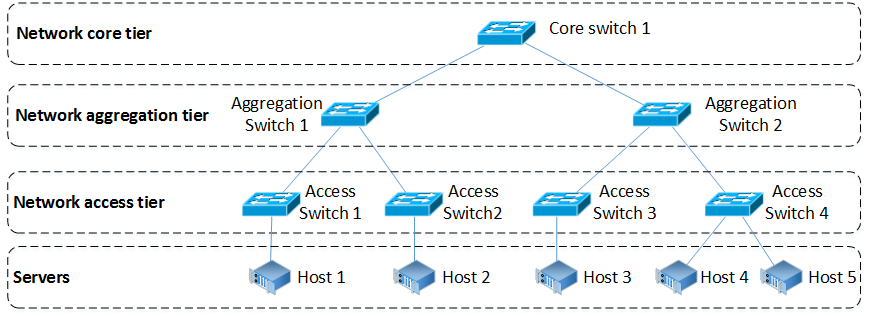
\includegraphics[scale=0.70]{network_topology}
	\caption{Typical datacenter topology}
	\label{fig:network_topology}
\end{figure}
%
\section{Elastic SDN controller cluster}
\label{section:functional-tests}
The first batch of tests carried out were functional tests, designed to validate the correctness of the implementation and the validity of the architecture.\\
%
For the validation of the \gls{SDN} controller elastic cluster described in Chapter \ref*{chapter:implementation} Section \ref{section:SDN-controller-cluster-implementation}, the correctness of such implementation greatly depended on the correctness of the Floodlight controller, and it is therefore considered that any behavior coherent with that of the base version of Floodlight is therefore correct.
Furthermore, all architecture-specific behavior must be validated with the requirements and desired behavior described in Chapter \ref*{chapter:architecture} Section \ref{section:SDN-controller-cluster}.\\
%
The request router, while partially implemented as stated in Section \ref{section:test-environment}, was also subject to testing to the remaining components that were implemented in the test environment.
The validation of the correctness of the request router is validated with the requirements and desired behavior described in Chapter \ref*{chapter:architecture} Section \ref{section:request-router} and implementation specific particularities indicated in Chapter \ref*{chapter:implementation} Section \ref{section:request-router-implementation}.
%
%
\subsection{Scenarios}
\label{subsection:functional-tests-scenarios}
For the \gls{SDN} controller elastic cluster specific functional tests, the scenarios to be tested are as follows:
\begin{enumerate}
	\item Validate cluster membership behavior, consistency and exchanged messages. To do so the first two controller instances are to be initiated simultaneously and let them form a cluster while monitoring the network for exchanged messages. After convergence has been reached, a third controller instance is to be introduced and let it join the cluster while still monitoring the network for exchanged messages.
	\item Validate \gls{MIB} consistency throughout the cluster and exchanged messages by manipulating the network topology to add, remove and simulate failure of OpenFlow switches and hosts as well as simulate switch management transference between available controller instances by provoking failure of cluster instances. The management network is to be monitored for exchanged messages throughout the tests.
	\item Validate the correct programming of OpenFlow switches. This functionality is to be validated by means of executing the module implemented as described in Chapter \ref*{chapter:implementation} Section \ref{subsection:poc-application} to allow \gls{TCP} connections between Host 1 and Host 3 as well as between Host 4 and Host 5. 
\end{enumerate}
%
For the request router specific functional tests, the key points tested are as follows:
\begin{enumerate}
	\item Validate request router clustering and state replication by having OpenFlow switches establish management connections to to the \gls{IPAddress} of the \gls{SDN} controller cluster and validating that both request router instances have the same connection state information.
	\item Validate that the component developed as described in Chapter \ref*{chapter:implementation} Section \ref{subsection:elastic-cluster-integration-implementation} properly integrates with the \gls{SDN} cluster as well as with \gls{LVS}'s ipvsadm tool by provoking \gls{SDN} controller cluster membership changes.
\end{enumerate}
%
\subsection{Results}
\label{section:functional-tests-results}
%
The results obtained from the execution of the functional tests on the experimental implementation show that the proposed architecture provides the desired properties and moreover that the implementation's behavior is coherent with that of the Floodlight.
Furthermore, the request router also complied with the specifications and expected implementation behavior.\\
%
Through the execution of the functional tests for the \gls{SDN} controller elastic cluster, it was found that all relevant network events such as switch, host, links registration/de-registration as well as inter-switch adjacencies are being correctly and timely detected and properly handled to update the local \gls{MIB} and trigger appropriate messages to peer cluster members, which also update their \gls{MIB} accordingly.
It was also confirmed that all messages described in Table \ref{table:cluster-message-spec} within the scope of cluster membership and targeting the whole cluster are sent using multicast, therefore keeping the desired group communication properties described in Chapter \ref*{chapter:architecture} Section \ref{section:SDN-controller-cluster}.\\
%
The functional tests to which the request router was subjected to were used to validate its correct behavior.
However, these tests also led to the discovery of a Master/Master cluster feature instead of the predicted Master/Slave cluster as per \gls{LVS}'s documentation.
%
\section{Distributed network policy module tests}
\label{section:performance-tests}
The use-case scenario of a global policy application that was previously functionally tested was also subject to performance benchmarking.
To that extent, the same scenario used to validate the correct programming of OpenFlow switches was also used to retrieve latency metrics for the programming process.
%
\subsection{Scenario}
\label{subsection:performance-tests-scenario}
Once again, this scenario specified the correct programming of the OpenFlow switches in order to allow for the establishment of \gls{TCP} connections between Host 1 and Host 3 as well as between Host 4 and Host 5.
To fully test the flow programming capabilities, Flow Entries were configured with matches for \gls{OSI} Layer 2, 3 and 4 source and destination fields as well as \gls{OSI} Layer 4 protocol number and physical port through which the traffic was being admitted into the network, coming to a total of 8 match fields per Flow Entry.\\
Since the tests were performed using \gls{TCP} connections, bi-directionality is implied, which means that for every \gls{TCP} session opened there will be two Flow Entries programmed in each of the involved OpenFlow switches.
For completeness purposes and in order to provide scalability metrics, these tests were performed using a two-instance controller cluster and repeated using a three-instance controller cluster, with OpenFlow switches evenly distributed among them by the request router component.
%
\subsection{Results}
\label{subsection:performance-tests-results}
%
The results obtained are stated in Tables \ref{table:perfomance-tests-2controllers} and \ref{table:perfomance-tests-3controllers} and plotted in Figure \ref{fig:performance}.
%
\begin{table}[h!]
	\begin{center}
		\rowcolors{2}{EvenRowColor}{OddRowColor}
		\begin{tabular}{ | c | c | c | }
			\rowcolor{HeaderRowColor}
			\hline
			\textbf{1 connection} & \textbf{5 Simultaneous connections} & \textbf{10 Simultaneous connections}\\
			\hline
			6207 milliseconds & 6618 milliseconds & 11714 milliseconds \\
			\hline
			6209 milliseconds & 6414 milliseconds & 14918 milliseconds \\
			\hline
			4406 milliseconds & 6614 milliseconds & 11270 milliseconds \\
			\hline
			4406 milliseconds & 6410 milliseconds & 11709 milliseconds \\
			\hline
			6406 milliseconds & 6609 milliseconds & 14919 milliseconds \\
			\hline
			6406 milliseconds & 6414 milliseconds & 11705 milliseconds \\
			\hline
			6406 milliseconds & 6413 milliseconds & 10725 milliseconds \\
			\hline
			6006 milliseconds & 6213 milliseconds & 10738 milliseconds \\
			\hline
			6206 milliseconds & 6609 milliseconds & 11722 milliseconds \\
			\hline
		\end{tabular}
		\caption{Flow programming results with a two-instance controller cluster}
		\label{table:perfomance-tests-2controllers}
	\end{center}
\end{table}
%
\begin{table}[h!]
	\begin{center}
		\rowcolors{2}{EvenRowColor}{OddRowColor}
		\begin{tabular}{ | c | c | c | }
			\rowcolor{HeaderRowColor}
			\hline
			\textbf{1 connection} & \textbf{5 Simultaneous connections} & \textbf{10 Simultaneous connections}\\
			\hline
			6606 milliseconds & 6614 milliseconds & 6681 milliseconds \\
			\hline
			6406 milliseconds & 6614 milliseconds & 6678 milliseconds \\
			\hline
			6206 milliseconds & 6610 milliseconds & 10686 milliseconds \\
			\hline
			6406 milliseconds & 6614 milliseconds & 6682 milliseconds \\
			\hline
			6206 milliseconds & 6414 milliseconds & 6685 milliseconds \\
			\hline
			6206 milliseconds & 6614 milliseconds & 10686 milliseconds \\
			\hline
			6406 milliseconds & 6618 milliseconds & 6690 milliseconds \\
			\hline
			6406 milliseconds & 6609 milliseconds & 10698 milliseconds \\
			\hline
			6006 milliseconds & 6610 milliseconds & 7092 milliseconds \\
			\hline
		\end{tabular}
		\caption{Flow programming results with a three-instance controller cluster}
		\label{table:perfomance-tests-3controllers}
	\end{center}
\end{table}
%
\begin{figure}
	\centering
	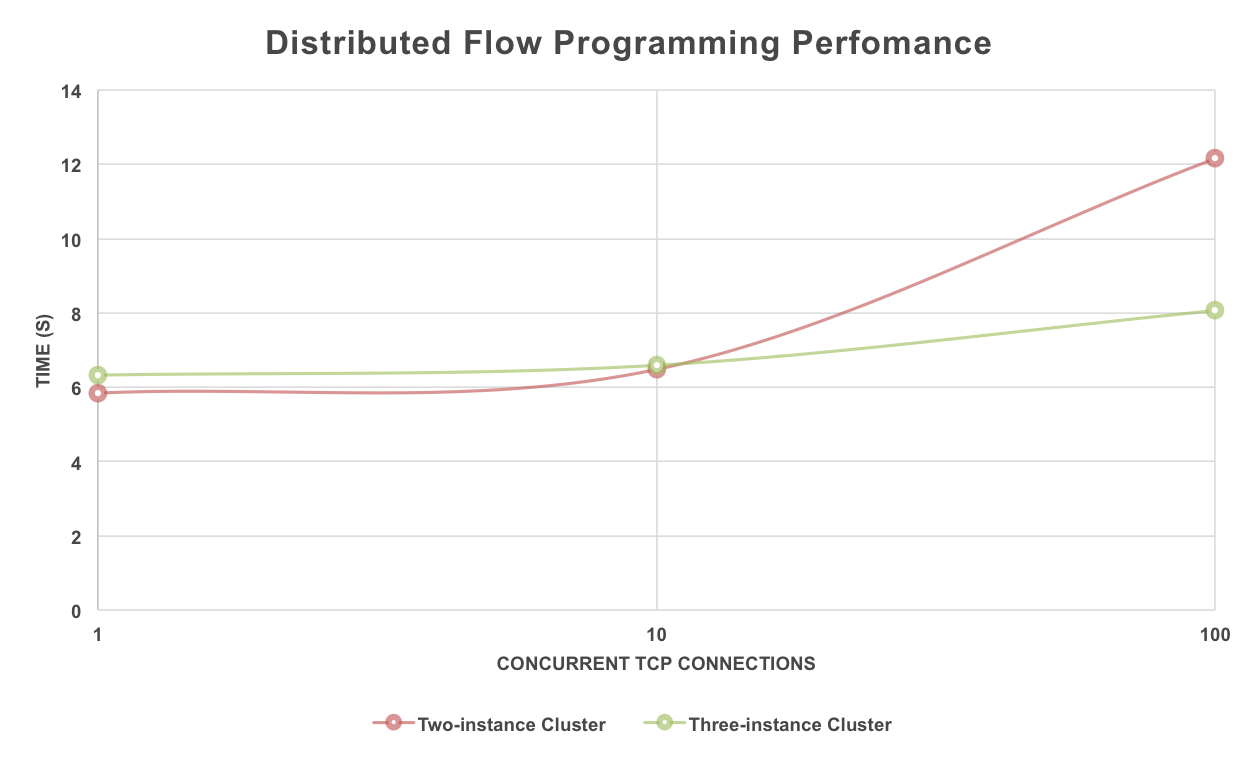
\includegraphics[scale=0.65]{performance_results.png}
	\caption{Performance indicators for the distributed network policy module}
	\label{fig:performance}
\end{figure}
%
\section{Analysis}
\label{section:considerations}
Due to Mininet's limitations, switches and hosts cannot be added or removed dynamically, however, they can be isolated from the network by shutting down all ports and in the particular case of switches removing configuration for controller connection.
It is not evident however that this limitation impacted the tests in anyway.\\
%
The results obtained from the tests to the \gls{SDN} controller elastic cluster showed that both cluster membership and \gls{MIB} are kept consistent throughout cluster members after adding, removing and provoking deliberate failures on controller instances as well as OpenFlow switches.\\
%
The results obtained while benchmarking the distributed network policy application also yielded positive results, showing that it is already possible to have a 33$\%$ efficiency increase by adding a third \gls{SDN} controller instance to the cluster when there are more than 10 concurrent \gls{TCP} sessions traversing the controlled network, thus achieving the desired scalability property.
However, if we take into account the absolute time required for the completion of flow configuration operations, the results obtained are unsatisfactory, which might be related to factors such as the overall load of the hardware supporting the test environment, virtualization overhead, network emulation environment overhead and finally to a suboptimal implementation of \gls{TCP} unicast connections between controller instances, which instead of caching connections between \gls{SDN} Controller instances for further communications are being opened and closed to send a single message.\\
The global memory footprint of the controller instances appear to have suffered an increase of approximately $10\%$ when executing the prototype Floodlight module.
